\documentclass[../main.tex]{subfiles}
 
\begin{document}
\chapter{The maximum entropy distribution: exponentially distributed component lifetimes}
\label{sec:common_distributions}
Suppose we have a series systems in which component lifetimes are exponentially 
distributed.

\section{Parametric functions}
Suppose the \jth component has a failure rate $\tparam{\lambda}_j$, denoted by 
$\cv_j \sim \text{EXP}(\tparam{\lambda}_j)$. The random variable $\cv_j$ has 
reliability, density, and failure rate functions given respectively by
\begin{align}
    \label{eq:expo_reliability}
    \srv_j(t \Given \tparam\lambda_j) &=
        \exp(-\tparam\lambda_j \cdot t)\,,\\
    \label{eq:expo_pdf}
    \pdf_j(t \Given \tparam\lambda_j) &=
        \tparam\lambda_j \exp(-\tparam\lambda_j \cdot t)\,,\\
    \label{eq:expo_haz}
    \haz_j(\cdot \Given \tparam\lambda_j) &=
        \tparam{\lambda}_j\,,
\end{align}
where $t > 0$ and $\tparam{\lambda}_j > 0$.

A series system with exponentially distributed lifetimes is also 
exponentially distributed.
\begin{theorem}
\label{thm:expo_series_family}
The random lifetime $\sv$ of a series system composed of $m$ components with 
exponentially distributed lifetimes is exponentially distributed with a failure 
rate that is the sum of the component failure rates with a true parameter index 
given by
\begin{equation}
    \tparam{\vec\lambda} = \Tuple{\tparam\lambda_1, \ldots, 
    \tparam\lambda_m}^{\Transpose}
\end{equation}
where $\tparam{\lambda}_j$ is the failure rate of the \jth component. That is,
\begin{equation}
    \sv \sim \expdist \left(\sum_{j=1}^{m} \tparam{\lambda}_j\right)\,,
\end{equation}

\end{theorem}
\begin{proof}
By \cref{thm:series_reliability_function},
\begin{equation}
    \srv_{\sv}(t \Given \tparam{\vec\lambda}) = \prod_{j=1}^{m} \srv_j(t \Given 
    \tparam\lambda_j)\,.
\end{equation}
Plugging in the component reliability functions as given by 
\cref{eq:expo_reliability} results in
\begin{equation}
    \srv_{\sv}(t \Given \tparam{\vec\lambda}) = \prod_{j=1}^{m} 
    \exp(-\tparam\lambda_j \cdot t) =
    \exp \left(-\left [ \sum_{j=1}^{m}{\tparam\lambda_j} \right ] t\right)\,.
\end{equation}
This reliability function belongs to the family of exponential 
distributions with a true parameter index given by the sum of the component 
failure rates.
\end{proof}

By \cref{thm:expo_series_family}, the system has a probability density, 
failure rate, and reliability functions given respectively by
\begin{align}
\label{eq:expo_sys_pdf}
\spdf(t \Given \tparam{\vec\lambda}) &=
    \left ( \sum_{j=1}^{m} {\tparam{\lambda}_j} \right ) \exp
    \left(-\left [ \sum_{j=1}^{m}{\tparam{\lambda_j}} \right ] t\right)\,,\\
\label{eq:expo_sys_failure_rate}
\haz_{\sv}(\cdot \Given \tparam{\vec\lambda}) &=
    \sum_{j=1}^{m}{\tparam\lambda_j}\,,\\
\label{eq:sys_expo_reliability_function}
\srv_{\sv} \left(t \Given \tparam{\vec\lambda} \right) &=
    \exp \left(-\left [ \sum_{j=1}^{m}{\tparam\lambda_j} \right ] t\right)
\end{align}
where $t > 0$ and $\tparam{\lambda}_j > 0$.

The conditional probability that component $k$ is the cause of a system failure at time $t$ is given by
\begin{equation}
\label{eq:expo_prob_K_given_S}
    \pmf_{\RV{K} \Given \sv}(k \Given t, \tparam{\vec\lambda}) = \pmf_{\RV{K}}(k \Given \tparam{\vec\lambda}) =
        \frac{\tparam{\lambda}_k}{\sum_{p=1}^{m} 
        \tparam{\lambda}_p}\SetIndicator{\Set{K}}(k)\,.
\end{equation}
\begin{proof}
By \cref{thm:series_failure_rate_function},
\begin{equation}
\pmf_{\RV{K} \Given \sv}(k \Given t, \tparam{\vec\lambda}) = \frac
    {\haz_k(t \Given \tparam{\vec\lambda}_k)}
    {\haz_{\sv}(t \Given \tparam{\vec\lambda})}\,.
\end{equation}
Plug in the failure rate of component $k$ and the failure rate of the system given by \cref{eq:expo_sys_failure_rate,eq:expo_haz}.
\end{proof}
Due to the constant failure rates of the components, $\RV{K}$ and $\sv$ are independent. The joint density of $\RV{K}$ and $\sv$ is given by
\begin{equation}
\label{eq:expo_joint_k_s}
\pdf_{\RV{K}, \sv}(k, t \Given \tparam{\vec\lambda}) =
    \tparam{\lambda}_k \exp \left(-\left [ \sum_{j=1}^{m}{\tparam{\lambda_j}} \right ] t\right)
    \SetIndicator{\Set{K} \times \RealSet^{+}}(k,t)
\end{equation}
\begin{proof}
By definition,
\begin{equation}
\pdf_{\RV{K}, \sv}(k, t \Given \tparam{\vec\lambda}) =
    \pmf_{\RV{K} \Given \sv}(k \Given t, \tparam{\vec\lambda}) \spdf(t \Given \tparam{\vec\lambda})\,.
\end{equation}
Plug in the conditional probability and the marginal probability given by \cref{eq:expo_prob_K_given_S,eq:expo_sys_pdf}.
\end{proof}

The conditional joint density of $\rvcand$ and $\sv$ given $\RV{W}$ is given by
\begin{equation}
    \jointpdf(\cand, t \Given w, \tparam{\vec\lambda}) = \frac{\SetIndicator{\RealSet_{>0} \times \candsw{w}}(t,\cand)}{\binom{m-1}{w-1}} \left ( \sum_{j \in \cand} \lambda_j \right ) \exp \left [ - \left ( \sum_{j=1}^{m} \lambda_j \right ) t \right ]\,,
\end{equation}
whose proof follows from \cref{thm:general_joint_likelihood_cand}.

The conditional probability that a component in $\rvcand$ is the cause of a system failure given that $\sv = t$ and $\RV{W} = w$ is given by
\begin{equation}
\label{eq:expo_cand_given_s}
    \pmf_{\rvcand \Given \sv, \RV{W}}(\cand \Given t, w, \tparam{\vec\lambda}) =
        \frac{ \sum_{j \in \cand} \tparam{\lambda}_j }
            { \binom{m-1}{w-1} \sum_{p=1}^{m} \tparam{\lambda}_p } \SetIndicator{\RealSet_{>0} \times \candsw{w}}(t,\cand)\,.
\end{equation}
whose proof follows from \cref{def:general_cond_cand_probability}.

Note that the marginal distribution of $\rvcand$ given $\RV{W}$ is given by
\begin{equation}
\label{eq:expo_cand_given_s}
     \pmf_{\rvcand \Given \RV{W}}\!\left(\cand \Given w, \tparam{\vec\lambda}\right) =
        \frac{ \sum_{j \in \cand} \tparam{\lambda}_j }
            { \binom{m-1}{w-1} \sum_{p=1}^{m} \tparam{\lambda}_p } \SetIndicator{\candsw{w}}(\cand)\,,
\end{equation}
\begin{proof}
The marginal is given by
\begin{align}
     \pmf_{\rvcand \Given \RV{W}}(\cand \Given w, \tparam{\vec\lambda})
        &= \int_{-\infty}^{\infty} \jointpdf\left(\cand, t \Given w, \tparam{\vec\lambda}\right) \dif t\\
        &= \int_{0}^{\infty} \mathsmaller{\frac{\SetIndicator{\RealSet_{+} \times \candsw{w}}(t,\cand)}{\binom{m-1}{w-1}}
        	\left ( \sum_{j \in \cand} \lambda_j \right ) \exp \left [ - \left ( \sum_{j=1}^{m} \lambda_j \right ) t \right ] \dif t}\\
        &= \mathsmaller{\frac{ \SetIndicator{\candsw{w}(\cand)}}{\binom{m-1}{w-1}}} \sum_{j \in \cand} \lambda_j \int_{0}^{\infty} \mathsmaller{ \exp \left [ - \left ( \sum_{j=1}^{m} \lambda_j \right ) t \right ] \dif t}\,.
\end{align}
Multiplying the integrand by
\begin{equation}
    \frac{\sum_{j=1}^{m} \lambda_j}{\sum_{j=1}^{m} \lambda_j}\,
\end{equation}
results in
\begin{align}
     \pmf_{\rvcand \Given \RV{W}}(\cand \Given w, \tparam{\vec\lambda})
        &= \mathsmaller{\frac{ \SetIndicator{\candsw{w}(\cand)} }{\binom{m-1}{w-1}} \frac{\sum_{j \in \cand} \lambda_j}{\sum_{j=1}^{m} \lambda_j}} \int_{0}^{\infty} \mathsmaller{ \left ( \sum_{j=1}^{m} \lambda_j \right) \exp \left [ - \left ( \sum_{j=1}^{m} \lambda_j \right ) t \right ] \dif t}\\
        &= \mathsmaller{\frac{ \SetIndicator{\candsw{w}(\cand)} }{\binom{m-1}{w-1}} \frac{\sum_{j \in \cand} \lambda_j}{\sum_{j=1}^{m} \lambda_j}} \int_{0}^{\infty} \spdf\left(t \Given \vec{\tparam\lambda}\right) \dif t\\
        &= \mathsmaller{\frac{ \SetIndicator{\candsw{w}(\cand)}}{\binom{m-1}{w-1}} \frac{\sum_{j \in \cand} \lambda_j}{\sum_{j=1}^{m} \lambda_j}}\,.
\end{align}
\end{proof}
The marginal distribution of $\rvcand \Given \RV{W} = w$ given by \cref{dummyref} is the same as the joint distribution of $\rvcand$ and $\sv$ given 
$\RV{W}$ given by \cref{eq:expo_cand_given_s}.
Thus, $\rvcand$ and $\sv$ are conditionally independent given $\RV{W}$.

\section{Maximum entropy distribution}
The larger the variance of the estimator, the larger a sample necessary to obtain an estimate with a given mean squared error.

Given that $\entropy(\RV{K} \Given \sv) \leq \entropy(\RV{K})$, a maximum entropy distribution has the form
\begin{equation}
\entropy(\RV{K}, \sv) = \entropy(\RV{K}) + \entropy(\sv)\,,
\end{equation}
where each of the components, and thus the system lifetime $\sv$, has an interval of support $(0,\infty)$.

Given the way in which $\RV{K}$ is defined as a function of $\sv$, there is a possibility that $\sv$ and $\RV{K}$ are necessarily dependent.
However, by \cref{?}, we see that if the component lifetimes are exponentially distributed, then the system lifetime $\sv$ is exponentially distributed, and by \cref{?} $\RV{K}$ is \emph{independent} of $\sv$.

Moreover, if we constrain the system lifetime to have an expectation $\mu$, then the maximum entropy distribution of $\sv$ is given by
\begin{equation}
\sv \sim \expdist(\lambda = 1 / \mu)\,.
\end{equation}

Independently, the maximum entropy distribution of the discrete random variable $\RV{K}$ is given by the discrete uniform distribution
\begin{equation}
\RV{K} \sim \unifdist(1,m)\,.
\end{equation}
By \cref{?}, we know that these components must be exponentially distributed and that each component must be uniformly distributed such the sum of their failure rates must equal $\lambda$, i.e.,
\begin{equation}
\cv_j \sim \expdist(\lambda / m)
\end{equation}
for $j=1,\ldots,m$.

TODO: fix this

The entropy of $\Pair{\sv}{\RV{K}}$ has very little to do determining the \emph{parameters}. The preceding discussion only applied to the number of questions, on average, needed to discern which component failed, and, independently, when did it fail, i.e., sample from $\RV{K}$ and then from $\sv$

% compare max entropy distribution against other exp dists that aren't max... 
%see asymptotics and such

\section{Maximum likelihood estimator}
According to \cref{def:general_mle}, the maximum likelihood estimator of $\tparam{\vec\lambda}$ is the value that maximizes the log-likelihood on a given masked system failure time sample, denoted $\mfs$. The likelihood function is given by
\begin{equation}
\label{eq:expo_like}
\likelihood(\vec\lambda \Given \mfs) \propto
    \exp \left [ - \left ( \sum_{j=1}^{m} \lambda_j \right ) \left ( \sum_{i=1}^{n} t_i \right ) \right ]
    \left [ \prod_{i=1}^{n} \left ( \sum_{j \in \cand_i} \lambda_j \right ) \right ]\,,
\end{equation}
whose proof follows from \cref{def:likelihood_func}. Therefore, the log-likelihood function $\ell$ is given by
\begin{equation}
    \ell(\vec{\lambda} \Given \mfs) = \text{const} + \sum_{i=1}^{n} \ln \left [ \sum_{j \in \cand_i} \lambda_j \right ] - \left [ \sum_{i=1}^{n} t_i \right ] \left [ \sum_{j=1}^{m} \lambda_j \right ]\,.
\end{equation}
Thus, maximum likelihood estimator of $\tparam{\vec\lambda}$ is given by
\begin{equation}
\label{eq:expo_sys_mle}
    \expomle = \argmax_{\vec\lambda > \vec{0}} \ell(\vec\lambda \Given \mfs)\,.
\end{equation}
The solution to \cref{eq:expo_sys_mle} must be a stationary point, i.e., a point at which the score function is zero. The \jth component of the score function is given by
\begin{equation}
\label{eq:score_expo_j}
    \frac{\partial \ell}{\partial \lambda_j} = 
    \sum_{i=1}^{n} \left ( \sum_{p \in \cand_i} \lambda_p \right )^{-1} \SetIndicator{\cand_i}(j) - \sum_{i=1}^{n} t_i\,.
\end{equation}

According to \cref{def:converge_in_dist}, the sampling distribution of $\expomle$ converges in distribution to a multivariate normal with a mean given by $\tparam{\vec\lambda}$ and a variance-covariance given by
\begin{equation}
    \frac{1}{n} \infomatrx^{-1}(\tparam{\vec\lambda})\,.
\end{equation}
Since $\tparam{\vec\lambda}$ is not known it may be approximated by
\begin{equation}
    \infomatrx^{-1}\left(\expomle\right)\,.
\end{equation}

The $(j,k)$-th element of the Fisher information matrix is given by
\begin{equation}
\label{eq:expo_info}
    \left [ \infomatrx(\tparam{\vec\lambda}) \right ]_{j k} =
        \frac
        {
            \sum_{\cand}
            \left [
                \left ( \sum_{p \in \cand} \tparam{\lambda}_p \right )^{-1}
                \SetIndicator{\cand \times \cand}(j,k)
            \right ]
        }
        {
            \binom{m-1}{w-1} \sum_{p=1}^{m} \tparam{\lambda}_p
        }\,.
\end{equation}
where the summation indexed by $\cand$ is over $\PS{\Set{K}}$.
\begin{proof}
By \cref{eq:info_matrix_el}, the $(j,k)$-th element of the information matrix is given by
\begin{equation}
\label{eq:proof_expo_info_1}
\begin{split}
    \left [ \infomatrx(\tparam{\vec\lambda}) \right ]_{i j}
    = - \sum_{\cand} \int_{0}^{\infty} &
        \eval
        {
            \md{}{2}{\lambda_i}{}{\lambda_j}{}
            \ln \jointpdf \left(\cand, t \Given w, \vectomat{\vec\lambda} \right)
        }_{\vec\lambda=\tparam{\vec\lambda}} 
        \cdot\\
        & \qquad \qquad \qquad \qquad \jointpdf \left(\cand, t \Given w, \vectomat{\tparam{\vec\lambda}} \right) \dif t\,,
\end{split}
\end{equation}
In the above equation, the second-order partial derivative of the log of the joint density is equivalent to the partial derivative with respect to the \kth parameter of the \jth component of the score, given by \cref{eq:score_expo_j}, conditioned on a masked system failure time sample of size $1$, denoted by $\mfs_1$. This mixed second-order partial derivative is given by
\begin{align}
    \frac{\partial{}}{\partial \lambda_k} \frac{\partial \ell}{\partial \lambda_j}
        &= \frac{\partial{}}{\partial \lambda_k} \left (
            \left [ \sum_{p \in \cand} \lambda_p \right ]^{-1}
            \SetIndicator{\cand}(j) - t \right )\\
    \label{eq:proof_expo_info_2}
        &= -\left ( \sum_{p \in \cand} \lambda_p \right )^{-2} \SetIndicator{\cand \times \cand}(j,k)\,.
\end{align}
Plugging in the joint density and substituting \cref{eq:proof_expo_info_2} into \cref{eq:proof_expo_info_1} results in
\begin{equation}
    \left [ \infomatrx(\tparam{\vec\lambda}) \right ]_{i j} =
    \sum_{\cand}
    \int_{0}^{\infty}
    \eval{
        \left ( \sum_{p \in \cand} \lambda_p \right )^{-2} \SetIndicator{\cand \times \cand}(p,k)
    }_{\vec\lambda = \vec{\tparam\lambda}}
    \frac{1}{\binom{m-1}{w-1}}
    \left ( \sum_{p \in \cand} \tparam\lambda_p \right ) \exp \left ( - \left [ \sum_{p=1}^{m} \tparam\lambda_p \right ] t \right )
     \dif t\,.
\end{equation}
Simplifying and rearranging results in
\begin{equation}
\label{eq:proof_expo_info_3}
    \left [ \infomatrx(\tparam{\vec\lambda}) \right ]_{i j} =
    \frac{1}{\binom{m-1}{w-1}}
    \sum_{\cand}
    \left ( \sum_{p \in \cand} \tparam\lambda_p \right )^{-1}
    \SetIndicator{\cand \times \in \cand}(p,k)
    \int_{0}^{\infty}
    \exp \left ( - \left [ \sum_{p=1}^{m} \tparam\lambda_p \right ] t \right ) 
     \dif t\,.
\end{equation}
Multiplying the integral by $\frac{\sum_{p=1}^{m} \tparam\lambda_p}{\sum_{p=1}^{m} \tparam\lambda_p}$ results in an integral of the form
\begin{equation}
    \int_{0}^{\infty} \frac{\sum_{p=1}^{m} \tparam\lambda_p}{\sum_{p=1}^{m} \tparam\lambda_p} \exp \left ( - \left [ \sum_{p=1}^{m} \tparam\lambda_p \right ] t \right ) 
     \dif t\,.
\end{equation}
Pulling the $\left(\sum_{p=1}^{m} \tparam\lambda_p\right)^{-1}$ constant out of the integrand results in
\begin{align}
    \frac{1}{\sum_{p=1}^{m} \tparam\lambda_p} \int_{0}^{\infty}
    \left ( \sum_{p=1}^{m} \tparam\lambda_p \right ) \exp \left ( - \left [ \sum_{p=1}^{m} \tparam\lambda_p \right ] t \right ) \dif t
    &= \frac{1}{\sum_{p=1}^{m} \tparam\lambda_p} \int_{0}^{\infty}
    \spdf(t \Given \tparam{\vec\lambda}) \dif t\\
\label{eq:proof_expo_info_4}
    &= \frac{1}{\sum_{p=1}^{m} \tparam\lambda_p}\,.
\end{align}
Substituting \cref{eq:proof_expo_info_4} into \cref{eq:proof_expo_info_3} results in
\begin{equation}
\label{eq:proof_expo_info_5}
    \left [ \infomatrx(\tparam{\vec\lambda}) \right ]_{i j} =
    \frac{1}{\binom{m-1}{w-1}}
    \sum_{\cand} \left\{
    \left ( \sum_{p \in \cand} \tparam\lambda_p \right )^{-1}
    \frac{1}{\sum_{p=1}^{m} \tparam\lambda_p} \SetIndicator{\cand \times \cand}(p,k) \right \}\,.
\end{equation}
\end{proof}

\subsection{Sufficient statistics}
\label{sec:expo_sufficient}
Consider a sample of $n$ masked system failure times denoted by $\mfso$. The mean system lifetime of the sample is given by
\begin{equation}
    \bar{t} = \frac{1}{n} \sum_{i=1}^{n} \ti_i\,.
\end{equation}
and another statistic, denoted by $\cntsymb$, is a dictionary of candidate set-frequency count pairs where a candidate set $\vec{k} \in \cands$ maps to its sample frequency and is given by
\begin{equation}
    \cntsymb_{\vec{k}} = \sum_{i=1}^{n} \SetIndicator{\vec{k}}(\cand_i)\,.
\end{equation}
Given a sample $\mfso$, the likelihood $\likelihood(\vec\lambda \Given \mfso)$ described by \cref{eq:expo_like} is the same as the likelihood given by
\begin{equation}
\likelihood(\vec\lambda \Given \bar t, \cntsymb) =
    \exp \left( -n \bar{t} \sum_{j=1}^{m} \lambda_j \right)
    \prod_{\cand \in \candsw{w}} \left ( \sum_{j \in \cand} \lambda_j \right )^{\cntsymb_{\cand}}\,,
\end{equation}
where $\candsw{w}$ is the set of all candidate sets of cardinality $w$.
\begin{proof}
The likelihood function $\likelihood$ with respect to a sample of $n$ masked system failure times is given by
\begin{equation*}
\likelihood(\vec\lambda \Given \mfso) \propto
    \exp \left [ - \left ( \sum_{j=1}^{m} \lambda_j \right ) \left ( \sum_{i=1}^{n} t_i \right ) \right ]
    \left [ \prod_{i=1}^{n} \left ( \sum_{j \in \cand_i} \lambda_j \right ) \right ]\tag{\ref{eq:expo_like} revisited}\,.
\end{equation*}
Substituting $\sum_{i=1}^{n} \ti_i$ in the above equation with the equivalent expression $n \bar{t}$ results in
\begin{equation}
\likelihood(\vec\lambda \Given \mfs) \propto
    \exp \left [ - n \bar{t} \sum_{j=1}^{m} \lambda_j \right ]
    \underbrace{
        \left [ \prod_{i=1}^{n} \left ( \sum_{j \in \cand_i} \lambda_j \right ) \right ]
    }_{A}\,.
\end{equation}
In the above equation, each unique set $\left(\lambda_{j_1} + \cdots + \lambda_{j_w}\right)$ in the product (labeled $A$) has multiplicity $\cntsymb_{\{\lambda_{j_1} \cdots \lambda_{j_w}\}}$, thus we may substitute this product with the equivalent product
\begin{equation}
    \prod_{\cand \in \candsw{w}} \left ( \sum_{j \in \cand} \lambda_j \right )^{\cntsymb_{\cand}}\,,
\end{equation}
where $\cand$ is over all unique candidate sets of cardinality $w$. The result of this substitution is given by
\begin{equation}
\likelihood(\vec\lambda \Given \bar{t}, \cntsymb) =
    \exp \left ( -n \bar{t} \sum_{j=1}^{m} \lambda_j \right )
    \prod_{\cand \in \candsw{w}} \left ( \sum_{j \in \cand} \lambda_j \right )^{\cntsymb_{\cand}}\,.
\end{equation}
\end{proof}

The statistics $\bar{t}$ and $\cntsymb$ are jointly sufficient for $\vec{\tparam\lambda}$
\begin{proof}
By the Fisher–Neyman factorization theorem, since $\likelihood$ given by \cref{eq:expo_like} can be factored as $\likelihood(\bar{t}, \cntsymb) = h(\bar{t}, \cntsymb) g(\bar{t}, \cntsymb)$, $\cntsymb$ and $\bar t$ are joint sufficient statistics for $\tparam{\vec\lambda}$.
\end{proof}

It may be helpful to consider the following example.
\begin{example}
Suppose we have a $3$-out-of-$3$ system with exponentially distributed component lifetimes.
If we are given a sample of $4$ masked system times,
\begin{equation}
    \mfsoi{4} = \left(
        \Pair{t_1 = 1}{\cand_1 = \{ 1, 2 \}},
        \Pair{t_2 = 1}{\cand_2 = \{ 1, 3 \}},
        \Pair{t_3 = 2}{\cand_3 = \{ 1, 2 \}},
        \Pair{t_4 = 2}{\cand_4 = \{ 1, 2 \}}
    \right)\,,
\end{equation}
then joint sufficient statics of $\vec{\tparam\lambda}$ are
\begin{align*}
    \bar t &= \frac{1 + 1 + 2 + 2}{4} = \frac{3}{2}\,,\\
    \cntsymb &= \{\cntsymb_{\{1,2\}} \mapsto 3\,,\cntsymb_{\{1,3\}} \mapsto 1\}\,.
\end{align*}
No additional information is needed to compute the likelihood of $\vec\lambda$ with respect to the given $\mfsn{4}$ sample.
\end{example}

The log-likelihood $\ell$ is given by
\begin{equation}
\ell(\sysparamvec \Given \bar t, \vec\cntsymb, w) =
    -n \bar t \left ( \sum_{j=1}^{m} \lambda_j \right ) +
    \sum_{\cand \in \candsw{w}} \cntsymb_{\cand} \ln
        \left ( \sum_{j \in \cand} \lambda_j \right )\,.
\end{equation}
To find the MLE $\estimator{\vec\lambda}_n$, we find the stationary points for $\lambda_1, \ldots, \lambda_m$ given by
\begin{equation}
    0   =  -n \bar t +
            \sum_{\cand \in \candsw{w}} \cntsymb_{\cand}
                \left (
                    \sum_{j \in \cand} \lambda_j
                \right )^{-1} \SetIndicator{\cand}(k)\;; k = 1, \ldots, m\,.
\end{equation}
The $(j, k)$-th element of the observed information matrix $\observed_n$ is given by
\begin{equation}
    \left [ \observed_n(\tparam{\vec\lambda} \vec\cntsymb) \right ]_{j k} =
        - \sum_{\cand \in \candsw{w}} \cntsymb_{\cand} \left( \sum_{i \in \cand} \tparam\lambda_i \right)^{-2} \SetIndicator{\cand \times \cand}(j,k)\,,
\end{equation}
which only depends on the statistic $\cntsymb$.

\section{Applications}

A $(1-\alpha) \cdot 100 \%$-confidence interval for $\tparam{\lambda}_j$ is 
given by
\begin{equation}
\estimator\lambda_j \raisebox{.2ex}{$\scriptstyle\pm$} z_{1-\alpha/2}
    \sqrt{\frac{1}{n} \left [ \infomatrx^{-1}(\vec{\estimator{\vec\lambda}_n}) \right ]_{j j}}\,.
\end{equation}


\section{Case study: 3-out-of-3 system}
The $3$-out-of-$3$ system's lifetime distribution functions are given by
\begin{align}
    \srv_{\sv}(t \Given \tparam{\vec\lambda}) &=
        \exp
        \left [
            -(\tparam{\lambda}_1 + \tparam{\lambda}_2 + \tparam{\lambda}_3) t
        \right ]\,,\\
    \spdf(t \Given \tparam{\vec\lambda}) &=
        (\tparam{\lambda}_1 + \tparam{\lambda}_2 + \tparam{\lambda}_3)
        \exp
        \left [
            -(\tparam{\lambda}_1 + \tparam{\lambda}_2 + \tparam{\lambda}_3) t
        \right ]\,,\\
    \haz_{\sv}(t \Given \tparam{\vec\lambda}) &= \tparam{\lambda}_1 + \tparam{\lambda}_2 + \tparam{\lambda}_3\,,
\end{align}
where $t > 0$, $\tparam\lambda_1 > 0$, $\tparam\lambda_2 > 0$, and $\tparam\lambda_3 > 0$.

\subsection{Sampling distributions of the maximum likelihood estimator}
\subsubsection{Component sets of size two}
If we condition on samples in which each observation consists of two 
candidates, $\RV{W} = \Card{\rvcand} = 2$, the likelihood function is 
given by
\begin{equation}
\begin{split}
    \likelihood(\vec\lambda \Given \bar{t}, \cntsymb) &= (\lambda_1 + \lambda_2)^{\cnt{1,2}} (\lambda_1 + \lambda_3)^{\cnt{1,3}} (\lambda_2 + \lambda_3)^{\cnt{2,3}} \exp\left(-n \bar{t} \left(\lambda_1 + \lambda_2 + \lambda_3\right)\right)
\end{split}
\end{equation}
and the log-likelihood function is given by
\begin{equation}
\begin{split}
    \ell(\vec\lambda \Given \bar{t}, \cntsymb) &= \cnt{1,2} \ln(\lambda_1 + \lambda_2) + \cnt{1,3} \ln(\lambda_1 + \lambda_3) + \\
        & \qquad \qquad \cnt{2,3} \ln(\lambda_2 + \lambda_3) - n \bar{t} (\lambda_1 + \lambda_2 + \lambda_3)\,.
\end{split}
\end{equation}
The maximum likelihood estimate $\expomle$ is given by the solving the system of equations in which the score is zero, $\score(\vec\lambda) = \vec{0}$, where the score is given by
\begin{equation}
\label{eq:score_expo}
    \score\left(\vec\lambda\right) = \colvec{3}
        {\frac{\cnt{1,2}}{\lambda_1 + \lambda_2} +  \frac{\cnt{1,3}}{\lambda_1 + \lambda_3}}
        {\frac{\cnt{1,2}}{\lambda_1 + \lambda_2} +  \frac{\cnt{2,3}}{\lambda_2 + \lambda_3}}
        {\frac{\cnt{1,3}}{\lambda_1 + \lambda_3} +  \frac{\cnt{2,3}}{\lambda_1 + \lambda_3}} -
        n \bar{t} \colvec{3}{1}{1}{1}\,.
\end{equation}
This has a closed form solution given by
\begin{equation}
    \expomle = \frac{1}{n \bar{t}} \colvec{3}
        {\cnt{1,2} + \cnt{1,3} - \cnt{2,3}}
        {\cnt{1,2} - \cnt{1,3} + \cnt{2,3}}
        {-\cnt{1,2} + \cnt{1,3} + \cnt{2,3}}\,.
\end{equation}
The information matrix is given by
\begin{equation}
\infomatrx \left ( \tparam{\vec\lambda} \right ) =
\frac{1}{2(\tparam{\lambda}_1 + \tparam{\lambda}_2 + \tparam{\lambda}_3)}
\left[
\begin{array}{ccc}
 \frac{1}{\tparam{\lambda}_1+\tparam{\lambda}_2}+\frac{1}{\tparam{\lambda}_1+\tparam{\lambda}_3}    & \frac{1}{\tparam{\lambda}_1+\tparam{\lambda}_2}                                                   & \frac{1}{\tparam{\lambda}_1+\tparam{\lambda}_3}\\
 \frac{1}{\tparam{\lambda}_1+\tparam\lambda _2}                                                            & \frac{1}{\tparam{\lambda}_1+\tparam{\lambda}_2}+\frac{1}{\tparam{\lambda}_2+\tparam{\lambda}_3}   & \frac{1}{\tparam{\lambda}_2+\tparam{\lambda}_3}\\
 \frac{1}{\tparam{\lambda}_1+\tparam{\lambda}_3}                                                    & \frac{1}{\tparam{\lambda}_2+\tparam{\lambda}_3}                                                   & \frac{1}{\tparam{\lambda}_1+\tparam{\lambda}_3}+\frac{1}{\tparam{\lambda}_2+\tparam{\lambda}_3}
\end{array}
\right]
\end{equation}

To derive the variance-covariance of the sampling distribution of $\expomle$ for a sample of $n$ masked system failure times, denoted by $\sampdexpo$, we take the inverse of $n \cdot \infomatrx \left(\tparam{\vec\lambda} \right)$ resulting in
\begin{equation}
    \var_{\tparam{\vec\lambda}}\!\left[\sampdexpo\right] = \frac{\tparam{\lambda}_1+\tparam{\lambda}_2+\tparam{\lambda}_3}{n}
    \left[
        \begin{array}{ccc}
         \tparam{\lambda}_1 +  \tparam{\lambda}_2 +  \tparam{\lambda}_3 & - \tparam{\lambda}_3 & - \tparam{\lambda}_2 \\
        -\tparam{\lambda}_3 &  \tparam{\lambda}_1 +  \tparam{\lambda}_2   + \tparam{\lambda}_3 & - \tparam{\lambda}_1 \\
        -\tparam{\lambda}_2 & -\tparam{\lambda}_1  & \tparam{\lambda}_1   + \tparam{\lambda}_2   + \tparam{\lambda}_3 \\
\end{array}
\right]\,.
\end{equation}
%For large $n$, the $(i,j)-\text{th}$ entry is given approximately by
%\begin{equation}
%    \left[\covmatrixn\right]_{i j} \approx
%    \frac{2\left(\cnt{1,2} + \cnt{1,3} + \cnt{2,3}\right) \left(
%        \cnt{1,2} + \cnt{1,3} + \cnt{2,3}\right)}
%        {n (n \bar{t})^2}\,.
%\end{equation}
By the asymptotic unbiasedness of $\expomle$, the asymptotic mean squared error is given by the trace of the variance-covariance matrix,
\begin{equation}
    \mse\left(\sampdexpo\right) = \frac{3(\tparam{\lambda}_1 +  \tparam{\lambda}_2 +  \tparam{\lambda}_3)^2}{n}\,.
\end{equation}

According to \cref{thm:approx_normal}, for a sufficiently large sample size $n$,
\begin{equation}
\label{eq:expo_mvn3}
    \sampdexpo \sim \mathrm{MVN}\biggl(\tparam{\vec\lambda}, \frac{1}{n}\infomatrx^{-1}(\tparam{\vec\lambda})\biggr)\,.
\end{equation}
Consequently, each time we observe a particular $\sampdexpo = \expomle$, we draw a random vector from the multivariate normal distribution given by \cref{eq:expo_mvn3}. Thus, an independent asymptotic $(1-\alpha) \cdot 100 \%$-confidence interval for $\tparam\lambda_j$ is given by
\begin{equation}
    \estimator{\lambda}_j \raisebox{.2ex}{$\scriptstyle\pm$} \frac{z_{1 - \alpha/2}}{\sqrt n}
    \left (
        \estimator{\lambda}_1 + \estimator{\lambda}_2 + \estimator{\lambda}_3
    \right)\,.
\end{equation}

\subsubsection{Component sets of size one}
If we condition on samples in which each observation consists of one candidate, $\RV{W} = \Card{\rvcand} = 1$, the likelihood function is given by
\begin{equation}
    \likelihood(\vec\lambda \Given \bar{t}, \cntsymb) = \lambda_1^{\cnt{1}} \lambda_2^{\cnt{2}} \lambda_3^{\cnt{3}} \exp\left(-n \bar{t} \left(\lambda_1 + \lambda_2 + \lambda_3\right)\right)
\end{equation}
and the log-likelihood function is given by
\begin{equation}
    \ell(\vec\lambda \Given \bar{t}, \cntsymb) = \cnt{1} \ln\lambda_1 + \cnt{2} \ln\lambda_2 + \cnt{3} \ln\lambda_3 - n \bar{t}\left(\lambda_1 + \lambda_2 + \lambda_3\right)\,.
\end{equation}
The maximum likelihood estimator is given by
\begin{equation}
    \expomle = \frac{1}{n \bar{t}} \colvec{3}
        {\cnt{1}}
        {\cnt{2}}
        {\cnt{3}}\,,
\end{equation}
and the information matrix is given by
\begin{equation}
\infomatrx \left ( \tparam{\vec\lambda} \right ) =
\frac{1}{\tparam{\lambda}_1 + \tparam{\lambda}_2 + \tparam{\lambda}_3}
\left[
\begin{array}{ccc}
    \frac{1}{\tparam{\lambda}_1} & 0                            & 0\\
    0                            & \frac{1}{\tparam{\lambda}_2} & 0\\
    0                            & 0                            & \frac{1}{\tparam{\lambda}_3}
\end{array}
\right]\,,
\end{equation}
and thus the variance-covariance matrix is given by
\begin{equation}
    \cov\left(\tparam{\vec\lambda}\right) = \frac{\tparam{\lambda}_1+\tparam{\lambda}_2+\tparam{\lambda}_3}{n}
    \left[
    \begin{array}{ccc}
        \tparam{\lambda}_1 & 0                  & 0\\
        0                  & \tparam{\lambda}_2 & 0\\
        0                  & 0                  & \tparam{\lambda}_3
    \end{array}
\right]\,.
\end{equation}
The asymptotic mean squared error is given by the trace of the variance-covariance matrix,
\begin{equation}
    \mse\left(\sampdexpo\right) = \frac{(\estimator{\lambda}_1 +  \estimator{\lambda}_2 +  \estimator{\lambda}_3)^2}{n}\,,
\end{equation}
which has three times less mean squared error than when conditioning on $\Card{\rvcand} = 2$. That is, an $\mfs$ sample in which each observation consists of one candidate has more information about $\vec{\tparam\lambda}$ than a sample in which each observation consists of two candidates.

The independent asymptotic $(1-\alpha) \cdot 100 \%$-confidence interval for $\tparam\lambda_j$ is given by
\begin{equation}
    \estimator{\lambda}_j \raisebox{.2ex}{$\scriptstyle\pm$} z_{1 - \alpha/2}
    \sqrt{
        \frac
        {
            \estimator{\lambda}_j \left(\estimator{\lambda}_1 + \estimator{\lambda}_2 + \estimator{\lambda}_3\right)
        }
        {n}
    }\,.
\end{equation}
By comparison, the confidence interval when conditioning on $\Card{\rvcand} = 2$ is
\begin{equation}
    \sqrt{
        \frac
        {
            \estimator{\lambda}_1 + \estimator{\lambda}_2 + \estimator{\lambda}_3
        }
        {
            \estimator{\lambda}_j
        }
    }
\end{equation}
as wide.

\subsubsection{Degenerate: component sets of size three}
The degenerate case is all components are candidates, $\RV{W} = \Card{\rvcand} = 3$. There is no maximum likelihood estimator $\vec{\estimator{\vec\lambda}_n}$. Rather, solving the equation results in the underspecified system given by
\begin{equation}
    \sum_{j=1}^{3} \estimator\lambda_j - \frac{1}{\bar{t}} = 0\,,
\end{equation}
where $\estimator\lambda_j > 0$ for $j=1,2,3$.

The solution set of this underspecified system is the equation of a plane bounded in the positive region as depicted in \cref{fig:plane_sol}. The plane has a normal vector given by
\begin{equation}
\label{eq:normal_plane_vec}
    \vec{n} = \Tuple{1,1,1}^\Transpose\,,
\end{equation}
which is independent of the statistic $\bar{t}$. Across multiple samples, the statistic $\bar{t}$ varies but the normal vector of the plane does not. Thus, the sampling distribution of the solution set will be a density over planes bounded in the positive region with a normal vector given by \cref{eq:normal_plane_vec}.

As $n$ goes to infinity, the probability that $\vec{\tparam\lambda}$ intersects the plane goes to $1$. This information may not be very useful, especially if the system lifetime $\sv$ has a small expected value (the area of the bounded plane is $1/\bar{t}^2$), but if this is the only information available, what is the best course of action? An unbiased estimator that asymptotically converges to $\vec{\tparam\lambda}$ is not possible, but we can minimize some other loss function. If we assume $\vec{\tparam\lambda}$ takes on any supported value with equal likelihood, then the estimate that minimizes the expected Euclidean distance from the projection of $\vec{\tparam\lambda}$ onto the plane of the solution set is given by
\begin{equation}
    \vec{\tilde\lambda_n} = \frac{1}{3 \bar{t}} \vec{n}\,.
\end{equation}

\begin{figure}
\caption{$\expomle$ solutions given three candidates}
\label{fig:plane_sol}
\centering
\begin{tikzpicture}[scale=4]
    \filldraw
    [
        draw=gray,
        fill=gray!5,
    ]
    (1,0,0) node[anchor=south west] {$\frac{1}{\bar{t}}$} --
    (0,1,0) node[anchor=south east] {$\frac{1}{\bar{t}}$} --
    (0,0,1) node[anchor=east] {$\frac{1}{\bar{t}}$} -- cycle;
    \draw (0,0,0) node{$\vec{0}$};
    \draw[dashed,->] (.05,0,0) -- (1.5,0,0) node[anchor=north east]{$\estimator\lambda_1$};
    \draw[dashed,->] (0,.05,0) -- (0,1.5,0) node[anchor=north west]{$\estimator\lambda_2$};
    \draw[dashed,->] (0,0,.1) -- (0,0,1.5) node[anchor=north west]{$\estimator\lambda_3$};
    \draw[->] (0,0,0) -- (1,1,1) node[above right] {$\vec{n} = 
    \Tuple{1,1,1}^\Transpose$};
    \draw[dotted,<-] (.2,.7,.1) -- (.4,1.1,0) node[above] {solution plane};
    \draw[black,fill=black] (.333,.333,.333) circle (.1ex);
    \draw[dotted,<-] (.333,.3,.333) -- (.333,-.15,.333) node[below] {optimal $\expomle = \frac{1}{3 \bar{t}} \vec{n}$};
\end{tikzpicture}
\end{figure}

\subsection{Rate of convergence to the asymptotic sampling distribution}
In this section, we evaluate how rapidly the sampling distribution of $\mle$ 
converges to the asymptotic distribution as given by \cref{dummyref}, a 
multivariate normal with a mean $\tparam\sysparamvec$ and a variance-covariance 
matrix $\frac{1}{n} \infomatrx^{-1}\left(\tparam\sysparamvec\right)$.

By \cref{eq:mse_mle_trace}, the asymptotic mean squared error of the maximum likelihood estimator $\mle$ is given by the trace of the variance-covariance matrix, $\mse = \frac{1}{n} \trace \left ( \infomatrx^{-1} \bigl(\tparam\sysparamvec\bigr) \right)$. An estimator of the mean squared error from a sample of $r$ maximum likelihood estimates is given by
\begin{equation}
\estimator{\mse}\left(\mlei{1}, \ldots, \mlei{r}\right) = \frac{1}{r} 
\sum_{i=1}^{r} \left( \mlei{i} - \tparam\sysparamvec \right)^\Transpose \left( 
\mlei{i} - \tparam\sysparamvec \right)\,.
\end{equation}
By generating $r$ masked system failure time of samples of size $n$, denoted by $\mfswn{1}{n}, \ldots, \mfswn{1}{r}$, and finding the corresponding maximum likelihood estimates, denoted by $\mlei{1}, \ldots, \mlei{r}$, we may estimate the mean squared error and compare the result against the asymptotic mean squared error. When we perform these steps for masked system failure time samples of size $n = 1,\ldots, N$, we may plot the rate of convergence.

The absolute difference between the mean squared error of the asymptotic covariance matrix and the ``true'' covariance matrix is given by
\begin{equation}
    | \mse - \estimator\mse |\,,
\end{equation}





***
Let's use a profile likelihood to look at how the likelihood function changes 
with respect to a parameter component. Say, for instance, the other cmoponents 
in the parameter are nuisance parameters, and we are really just interested in 
the \jth component.
***



Let $\tparam{\vec\lambda} = \Tuple{2,3,4}^\Transpose$ and let the sample of 
masked system failure times be of size $n=1000$. Theoretically, the MLE 
$\vec{\estimator{\vec\lambda}_{1000}}$ is approximately distrubted as
\begin{equation}
\label{eq:expo_mvn_2_3_4}
    \vec{\estimator{\lambda}_{1000}} \sim \mathrm{MVN} \bigg ( 
    \Tuple{2,3,4}^\Transpose, \covn{1000} \bigg )\,.
\end{equation}
where
\begin{equation}
    \covn{1000} =
    \left(
        \begin{array}{ccc}
            0.081	&   -0.036  &   -0.027\\
            -0.036  &   0.081   &   -0.018\\
            -0.027  &   -0.018  &   0.081
        \end{array}
    \right)\,.
\end{equation}

We generated two different sets of data points, one from the theoretical distribution described in \cref{eq:expo_mvn_2_3_4} and the other from the maximum likelihood method applied to $\mfsn{1000}$ samples. Refer to \cref{fig:theory_vs_actual} for a visualization of the data points. Visually, they have a similar distribution of data points, indicating that the asymptotic distribution is a reasonable approximation of the sampling distribution of the MLE $\vec{\estimator{\vec\lambda}_{1000}}$.
\begin{figure}
\centering
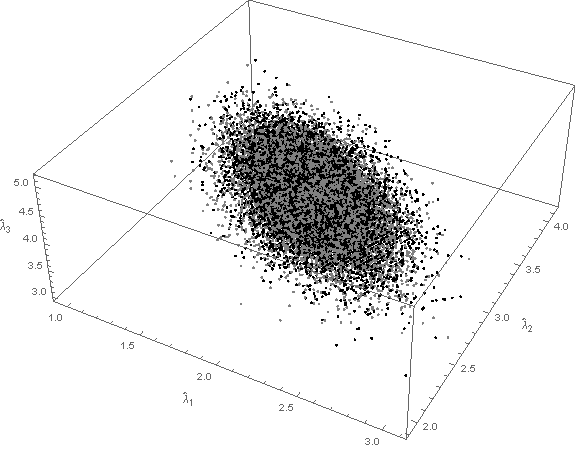
\includegraphics[width=0.5\linewidth]{superimposed.png}
\captionof{figure}{Theoretical MLE data points (gray) vs actual MLE data points (black)}
\label{fig:theory_vs_actual}
\end{figure}

A sample variance-covariance matrix of $r=10000$ maximum likelihood estimates 
was computed to be
\begin{equation}
    \widehat{\covn{1000}} =
    \left(
        \begin{array}{ccc}
            0.081  &   -0.037 &   -0.027\\
            -0.037 &   0.082  &   -0.018\\
            -0.027 &   -0.018 &   0.081
        \end{array}
    \right)\,,
\end{equation}
which is approximately equivalent to the theoretical asymptotic distribution given by \cref{eq:expo_mvn_2_3_4}.

\begin{figure}
\begin{center}
% GNUPLOT: LaTeX picture
\setlength{\unitlength}{0.240900pt}
\ifx\plotpoint\undefined\newsavebox{\plotpoint}\fi
\sbox{\plotpoint}{\rule[-0.200pt]{0.400pt}{0.400pt}}%
\begin{picture}(1500,900)(0,0)
\sbox{\plotpoint}{\rule[-0.200pt]{0.400pt}{0.400pt}}%
\put(250.0,131.0){\rule[-0.200pt]{4.818pt}{0.400pt}}
\put(230,131){\makebox(0,0)[r]{0.0000001}}
\put(1419.0,131.0){\rule[-0.200pt]{4.818pt}{0.400pt}}
\put(250.0,155.0){\rule[-0.200pt]{2.409pt}{0.400pt}}
\put(1429.0,155.0){\rule[-0.200pt]{2.409pt}{0.400pt}}
\put(250.0,186.0){\rule[-0.200pt]{2.409pt}{0.400pt}}
\put(1429.0,186.0){\rule[-0.200pt]{2.409pt}{0.400pt}}
\put(250.0,202.0){\rule[-0.200pt]{2.409pt}{0.400pt}}
\put(1429.0,202.0){\rule[-0.200pt]{2.409pt}{0.400pt}}
\put(250.0,210.0){\rule[-0.200pt]{4.818pt}{0.400pt}}
\put(230,210){\makebox(0,0)[r]{0.0000010}}
\put(1419.0,210.0){\rule[-0.200pt]{4.818pt}{0.400pt}}
\put(250.0,233.0){\rule[-0.200pt]{2.409pt}{0.400pt}}
\put(1429.0,233.0){\rule[-0.200pt]{2.409pt}{0.400pt}}
\put(250.0,265.0){\rule[-0.200pt]{2.409pt}{0.400pt}}
\put(1429.0,265.0){\rule[-0.200pt]{2.409pt}{0.400pt}}
\put(250.0,281.0){\rule[-0.200pt]{2.409pt}{0.400pt}}
\put(1429.0,281.0){\rule[-0.200pt]{2.409pt}{0.400pt}}
\put(250.0,289.0){\rule[-0.200pt]{4.818pt}{0.400pt}}
\put(230,289){\makebox(0,0)[r]{0.0000100}}
\put(1419.0,289.0){\rule[-0.200pt]{4.818pt}{0.400pt}}
\put(250.0,312.0){\rule[-0.200pt]{2.409pt}{0.400pt}}
\put(1429.0,312.0){\rule[-0.200pt]{2.409pt}{0.400pt}}
\put(250.0,344.0){\rule[-0.200pt]{2.409pt}{0.400pt}}
\put(1429.0,344.0){\rule[-0.200pt]{2.409pt}{0.400pt}}
\put(250.0,360.0){\rule[-0.200pt]{2.409pt}{0.400pt}}
\put(1429.0,360.0){\rule[-0.200pt]{2.409pt}{0.400pt}}
\put(250.0,367.0){\rule[-0.200pt]{4.818pt}{0.400pt}}
\put(230,367){\makebox(0,0)[r]{0.0001000}}
\put(1419.0,367.0){\rule[-0.200pt]{4.818pt}{0.400pt}}
\put(250.0,391.0){\rule[-0.200pt]{2.409pt}{0.400pt}}
\put(1429.0,391.0){\rule[-0.200pt]{2.409pt}{0.400pt}}
\put(250.0,422.0){\rule[-0.200pt]{2.409pt}{0.400pt}}
\put(1429.0,422.0){\rule[-0.200pt]{2.409pt}{0.400pt}}
\put(250.0,438.0){\rule[-0.200pt]{2.409pt}{0.400pt}}
\put(1429.0,438.0){\rule[-0.200pt]{2.409pt}{0.400pt}}
\put(250.0,446.0){\rule[-0.200pt]{4.818pt}{0.400pt}}
\put(230,446){\makebox(0,0)[r]{0.0010000}}
\put(1419.0,446.0){\rule[-0.200pt]{4.818pt}{0.400pt}}
\put(250.0,470.0){\rule[-0.200pt]{2.409pt}{0.400pt}}
\put(1429.0,470.0){\rule[-0.200pt]{2.409pt}{0.400pt}}
\put(250.0,501.0){\rule[-0.200pt]{2.409pt}{0.400pt}}
\put(1429.0,501.0){\rule[-0.200pt]{2.409pt}{0.400pt}}
\put(250.0,517.0){\rule[-0.200pt]{2.409pt}{0.400pt}}
\put(1429.0,517.0){\rule[-0.200pt]{2.409pt}{0.400pt}}
\put(250.0,525.0){\rule[-0.200pt]{4.818pt}{0.400pt}}
\put(230,525){\makebox(0,0)[r]{0.0100000}}
\put(1419.0,525.0){\rule[-0.200pt]{4.818pt}{0.400pt}}
\put(250.0,548.0){\rule[-0.200pt]{2.409pt}{0.400pt}}
\put(1429.0,548.0){\rule[-0.200pt]{2.409pt}{0.400pt}}
\put(250.0,580.0){\rule[-0.200pt]{2.409pt}{0.400pt}}
\put(1429.0,580.0){\rule[-0.200pt]{2.409pt}{0.400pt}}
\put(250.0,596.0){\rule[-0.200pt]{2.409pt}{0.400pt}}
\put(1429.0,596.0){\rule[-0.200pt]{2.409pt}{0.400pt}}
\put(250.0,604.0){\rule[-0.200pt]{4.818pt}{0.400pt}}
\put(230,604){\makebox(0,0)[r]{0.1000000}}
\put(1419.0,604.0){\rule[-0.200pt]{4.818pt}{0.400pt}}
\put(250.0,627.0){\rule[-0.200pt]{2.409pt}{0.400pt}}
\put(1429.0,627.0){\rule[-0.200pt]{2.409pt}{0.400pt}}
\put(250.0,659.0){\rule[-0.200pt]{2.409pt}{0.400pt}}
\put(1429.0,659.0){\rule[-0.200pt]{2.409pt}{0.400pt}}
\put(250.0,675.0){\rule[-0.200pt]{2.409pt}{0.400pt}}
\put(1429.0,675.0){\rule[-0.200pt]{2.409pt}{0.400pt}}
\put(250.0,682.0){\rule[-0.200pt]{4.818pt}{0.400pt}}
\put(230,682){\makebox(0,0)[r]{1.0000000}}
\put(1419.0,682.0){\rule[-0.200pt]{4.818pt}{0.400pt}}
\put(250.0,706.0){\rule[-0.200pt]{2.409pt}{0.400pt}}
\put(1429.0,706.0){\rule[-0.200pt]{2.409pt}{0.400pt}}
\put(250.0,737.0){\rule[-0.200pt]{2.409pt}{0.400pt}}
\put(1429.0,737.0){\rule[-0.200pt]{2.409pt}{0.400pt}}
\put(250.0,753.0){\rule[-0.200pt]{2.409pt}{0.400pt}}
\put(1429.0,753.0){\rule[-0.200pt]{2.409pt}{0.400pt}}
\put(250.0,761.0){\rule[-0.200pt]{4.818pt}{0.400pt}}
\put(230,761){\makebox(0,0)[r]{10.0000000}}
\put(1419.0,761.0){\rule[-0.200pt]{4.818pt}{0.400pt}}
\put(250.0,131.0){\rule[-0.200pt]{0.400pt}{4.818pt}}
\put(250,90){\makebox(0,0){$10$}}
\put(250.0,756.0){\rule[-0.200pt]{0.400pt}{4.818pt}}
\put(369.0,131.0){\rule[-0.200pt]{0.400pt}{2.409pt}}
\put(369.0,766.0){\rule[-0.200pt]{0.400pt}{2.409pt}}
\put(439.0,131.0){\rule[-0.200pt]{0.400pt}{2.409pt}}
\put(439.0,766.0){\rule[-0.200pt]{0.400pt}{2.409pt}}
\put(489.0,131.0){\rule[-0.200pt]{0.400pt}{2.409pt}}
\put(489.0,766.0){\rule[-0.200pt]{0.400pt}{2.409pt}}
\put(527.0,131.0){\rule[-0.200pt]{0.400pt}{2.409pt}}
\put(527.0,766.0){\rule[-0.200pt]{0.400pt}{2.409pt}}
\put(558.0,131.0){\rule[-0.200pt]{0.400pt}{2.409pt}}
\put(558.0,766.0){\rule[-0.200pt]{0.400pt}{2.409pt}}
\put(585.0,131.0){\rule[-0.200pt]{0.400pt}{2.409pt}}
\put(585.0,766.0){\rule[-0.200pt]{0.400pt}{2.409pt}}
\put(608.0,131.0){\rule[-0.200pt]{0.400pt}{2.409pt}}
\put(608.0,766.0){\rule[-0.200pt]{0.400pt}{2.409pt}}
\put(628.0,131.0){\rule[-0.200pt]{0.400pt}{2.409pt}}
\put(628.0,766.0){\rule[-0.200pt]{0.400pt}{2.409pt}}
\put(646.0,131.0){\rule[-0.200pt]{0.400pt}{4.818pt}}
\put(646,90){\makebox(0,0){$100$}}
\put(646.0,756.0){\rule[-0.200pt]{0.400pt}{4.818pt}}
\put(766.0,131.0){\rule[-0.200pt]{0.400pt}{2.409pt}}
\put(766.0,766.0){\rule[-0.200pt]{0.400pt}{2.409pt}}
\put(835.0,131.0){\rule[-0.200pt]{0.400pt}{2.409pt}}
\put(835.0,766.0){\rule[-0.200pt]{0.400pt}{2.409pt}}
\put(885.0,131.0){\rule[-0.200pt]{0.400pt}{2.409pt}}
\put(885.0,766.0){\rule[-0.200pt]{0.400pt}{2.409pt}}
\put(923.0,131.0){\rule[-0.200pt]{0.400pt}{2.409pt}}
\put(923.0,766.0){\rule[-0.200pt]{0.400pt}{2.409pt}}
\put(955.0,131.0){\rule[-0.200pt]{0.400pt}{2.409pt}}
\put(955.0,766.0){\rule[-0.200pt]{0.400pt}{2.409pt}}
\put(981.0,131.0){\rule[-0.200pt]{0.400pt}{2.409pt}}
\put(981.0,766.0){\rule[-0.200pt]{0.400pt}{2.409pt}}
\put(1004.0,131.0){\rule[-0.200pt]{0.400pt}{2.409pt}}
\put(1004.0,766.0){\rule[-0.200pt]{0.400pt}{2.409pt}}
\put(1025.0,131.0){\rule[-0.200pt]{0.400pt}{2.409pt}}
\put(1025.0,766.0){\rule[-0.200pt]{0.400pt}{2.409pt}}
\put(1043.0,131.0){\rule[-0.200pt]{0.400pt}{4.818pt}}
\put(1043,90){\makebox(0,0){$1000$}}
\put(1043.0,756.0){\rule[-0.200pt]{0.400pt}{4.818pt}}
\put(1162.0,131.0){\rule[-0.200pt]{0.400pt}{2.409pt}}
\put(1162.0,766.0){\rule[-0.200pt]{0.400pt}{2.409pt}}
\put(1232.0,131.0){\rule[-0.200pt]{0.400pt}{2.409pt}}
\put(1232.0,766.0){\rule[-0.200pt]{0.400pt}{2.409pt}}
\put(1281.0,131.0){\rule[-0.200pt]{0.400pt}{2.409pt}}
\put(1281.0,766.0){\rule[-0.200pt]{0.400pt}{2.409pt}}
\put(1320.0,131.0){\rule[-0.200pt]{0.400pt}{2.409pt}}
\put(1320.0,766.0){\rule[-0.200pt]{0.400pt}{2.409pt}}
\put(1351.0,131.0){\rule[-0.200pt]{0.400pt}{2.409pt}}
\put(1351.0,766.0){\rule[-0.200pt]{0.400pt}{2.409pt}}
\put(1378.0,131.0){\rule[-0.200pt]{0.400pt}{2.409pt}}
\put(1378.0,766.0){\rule[-0.200pt]{0.400pt}{2.409pt}}
\put(1401.0,131.0){\rule[-0.200pt]{0.400pt}{2.409pt}}
\put(1401.0,766.0){\rule[-0.200pt]{0.400pt}{2.409pt}}
\put(1421.0,131.0){\rule[-0.200pt]{0.400pt}{2.409pt}}
\put(1421.0,766.0){\rule[-0.200pt]{0.400pt}{2.409pt}}
\put(1439.0,131.0){\rule[-0.200pt]{0.400pt}{4.818pt}}
\put(1439,90){\makebox(0,0){$10000$}}
\put(1439.0,756.0){\rule[-0.200pt]{0.400pt}{4.818pt}}
\put(250.0,131.0){\rule[-0.200pt]{0.400pt}{155.380pt}}
\put(250.0,131.0){\rule[-0.200pt]{286.430pt}{0.400pt}}
\put(1439.0,131.0){\rule[-0.200pt]{0.400pt}{155.380pt}}
\put(250.0,776.0){\rule[-0.200pt]{286.430pt}{0.400pt}}
\put(844,29){\makebox(0,0){Sample size $n$}}
\put(844,838){\makebox(0,0){Mean squared error: difference between simulated vs asymptotic}}
\put(1279,735){\makebox(0,0)[r]{Absolute difference}}
\put(250,734){\makebox(0,0){$+$}}
\put(266,727){\makebox(0,0){$+$}}
\put(281,721){\makebox(0,0){$+$}}
\put(295,714){\makebox(0,0){$+$}}
\put(308,708){\makebox(0,0){$+$}}
\put(320,703){\makebox(0,0){$+$}}
\put(331,699){\makebox(0,0){$+$}}
\put(341,694){\makebox(0,0){$+$}}
\put(351,690){\makebox(0,0){$+$}}
\put(360,686){\makebox(0,0){$+$}}
\put(369,682){\makebox(0,0){$+$}}
\put(378,679){\makebox(0,0){$+$}}
\put(386,675){\makebox(0,0){$+$}}
\put(393,673){\makebox(0,0){$+$}}
\put(401,669){\makebox(0,0){$+$}}
\put(408,666){\makebox(0,0){$+$}}
\put(414,662){\makebox(0,0){$+$}}
\put(421,661){\makebox(0,0){$+$}}
\put(427,658){\makebox(0,0){$+$}}
\put(433,655){\makebox(0,0){$+$}}
\put(439,652){\makebox(0,0){$+$}}
\put(445,651){\makebox(0,0){$+$}}
\put(450,649){\makebox(0,0){$+$}}
\put(456,646){\makebox(0,0){$+$}}
\put(461,643){\makebox(0,0){$+$}}
\put(466,642){\makebox(0,0){$+$}}
\put(470,640){\makebox(0,0){$+$}}
\put(475,638){\makebox(0,0){$+$}}
\put(480,636){\makebox(0,0){$+$}}
\put(484,635){\makebox(0,0){$+$}}
\put(489,634){\makebox(0,0){$+$}}
\put(493,630){\makebox(0,0){$+$}}
\put(497,630){\makebox(0,0){$+$}}
\put(501,627){\makebox(0,0){$+$}}
\put(505,625){\makebox(0,0){$+$}}
\put(509,624){\makebox(0,0){$+$}}
\put(513,624){\makebox(0,0){$+$}}
\put(516,622){\makebox(0,0){$+$}}
\put(520,619){\makebox(0,0){$+$}}
\put(524,618){\makebox(0,0){$+$}}
\put(527,617){\makebox(0,0){$+$}}
\put(558,604){\makebox(0,0){$+$}}
\put(585,592){\makebox(0,0){$+$}}
\put(608,582){\makebox(0,0){$+$}}
\put(628,579){\makebox(0,0){$+$}}
\put(646,568){\makebox(0,0){$+$}}
\put(663,562){\makebox(0,0){$+$}}
\put(678,556){\makebox(0,0){$+$}}
\put(691,550){\makebox(0,0){$+$}}
\put(704,543){\makebox(0,0){$+$}}
\put(716,539){\makebox(0,0){$+$}}
\put(727,536){\makebox(0,0){$+$}}
\put(738,536){\makebox(0,0){$+$}}
\put(748,527){\makebox(0,0){$+$}}
\put(757,530){\makebox(0,0){$+$}}
\put(766,521){\makebox(0,0){$+$}}
\put(774,518){\makebox(0,0){$+$}}
\put(782,516){\makebox(0,0){$+$}}
\put(790,504){\makebox(0,0){$+$}}
\put(797,509){\makebox(0,0){$+$}}
\put(804,501){\makebox(0,0){$+$}}
\put(835,495){\makebox(0,0){$+$}}
\put(885,462){\makebox(0,0){$+$}}
\put(923,452){\makebox(0,0){$+$}}
\put(955,450){\makebox(0,0){$+$}}
\put(981,429){\makebox(0,0){$+$}}
\put(1004,433){\makebox(0,0){$+$}}
\put(1025,403){\makebox(0,0){$+$}}
\put(1043,417){\makebox(0,0){$+$}}
\put(1112,371){\makebox(0,0){$+$}}
\put(1162,396){\makebox(0,0){$+$}}
\put(1200,326){\makebox(0,0){$+$}}
\put(1232,350){\makebox(0,0){$+$}}
\put(1258,323){\makebox(0,0){$+$}}
\put(1281,290){\makebox(0,0){$+$}}
\put(1302,291){\makebox(0,0){$+$}}
\put(1351,257){\makebox(0,0){$+$}}
\put(1378,306){\makebox(0,0){$+$}}
\put(1421,298){\makebox(0,0){$+$}}
\put(1439,210){\makebox(0,0){$+$}}
\put(1349,735){\makebox(0,0){$+$}}
\put(250,727){\usebox{\plotpoint}}
\put(250.00,727.00){\usebox{\plotpoint}}
\put(269.16,719.02){\usebox{\plotpoint}}
\put(288.32,711.03){\usebox{\plotpoint}}
\put(307.74,703.75){\usebox{\plotpoint}}
\put(326.96,695.93){\usebox{\plotpoint}}
\put(346.12,687.95){\usebox{\plotpoint}}
\put(365.48,680.51){\usebox{\plotpoint}}
\put(384.76,672.85){\usebox{\plotpoint}}
\put(403.92,664.87){\usebox{\plotpoint}}
\put(423.22,657.26){\usebox{\plotpoint}}
\put(442.56,649.77){\usebox{\plotpoint}}
\put(461.72,641.78){\usebox{\plotpoint}}
\put(480.96,634.01){\usebox{\plotpoint}}
\put(500.36,626.68){\usebox{\plotpoint}}
\put(519.52,618.70){\usebox{\plotpoint}}
\put(538.70,610.77){\usebox{\plotpoint}}
\put(558.16,603.60){\usebox{\plotpoint}}
\put(577.32,595.62){\usebox{\plotpoint}}
\put(596.48,587.63){\usebox{\plotpoint}}
\put(615.96,580.52){\usebox{\plotpoint}}
\put(635.12,572.53){\usebox{\plotpoint}}
\put(654.28,564.55){\usebox{\plotpoint}}
\put(673.76,557.43){\usebox{\plotpoint}}
\put(692.92,549.45){\usebox{\plotpoint}}
\put(712.08,541.47){\usebox{\plotpoint}}
\put(731.56,534.35){\usebox{\plotpoint}}
\put(750.72,526.37){\usebox{\plotpoint}}
\put(769.99,518.67){\usebox{\plotpoint}}
\put(789.37,511.26){\usebox{\plotpoint}}
\put(808.52,503.28){\usebox{\plotpoint}}
\put(827.73,495.42){\usebox{\plotpoint}}
\put(847.27,488.44){\usebox{\plotpoint}}
\put(866.47,480.56){\usebox{\plotpoint}}
\put(885.63,472.57){\usebox{\plotpoint}}
\put(905.11,465.45){\usebox{\plotpoint}}
\put(924.27,457.47){\usebox{\plotpoint}}
\put(943.43,449.49){\usebox{\plotpoint}}
\put(962.91,442.37){\usebox{\plotpoint}}
\put(982.07,434.39){\usebox{\plotpoint}}
\put(1001.23,426.40){\usebox{\plotpoint}}
\put(1020.71,419.29){\usebox{\plotpoint}}
\put(1039.87,411.30){\usebox{\plotpoint}}
\put(1059.03,403.32){\usebox{\plotpoint}}
\put(1078.50,396.17){\usebox{\plotpoint}}
\put(1097.67,388.22){\usebox{\plotpoint}}
\put(1116.83,380.24){\usebox{\plotpoint}}
\put(1136.24,372.92){\usebox{\plotpoint}}
\put(1155.47,365.14){\usebox{\plotpoint}}
\put(1174.63,357.15){\usebox{\plotpoint}}
\put(1193.98,349.67){\usebox{\plotpoint}}
\put(1213.27,342.05){\usebox{\plotpoint}}
\put(1232.43,334.07){\usebox{\plotpoint}}
\put(1251.72,326.43){\usebox{\plotpoint}}
\put(1271.07,318.97){\usebox{\plotpoint}}
\put(1290.23,310.99){\usebox{\plotpoint}}
\put(1309.71,303.87){\usebox{\plotpoint}}
\put(1328.87,295.89){\usebox{\plotpoint}}
\put(1348.03,287.90){\usebox{\plotpoint}}
\put(1367.52,280.79){\usebox{\plotpoint}}
\put(1386.67,272.80){\usebox{\plotpoint}}
\put(1405.83,264.82){\usebox{\plotpoint}}
\put(1425.27,257.58){\usebox{\plotpoint}}
\put(1439,252){\usebox{\plotpoint}}
\sbox{\plotpoint}{\rule[-0.400pt]{0.800pt}{0.800pt}}%
\sbox{\plotpoint}{\rule[-0.200pt]{0.400pt}{0.400pt}}%
\put(1279,694){\makebox(0,0)[r]{Relative difference}}
\sbox{\plotpoint}{\rule[-0.400pt]{0.800pt}{0.800pt}}%
\put(250,641){\makebox(0,0){$\ast$}}
\put(266,638){\makebox(0,0){$\ast$}}
\put(281,636){\makebox(0,0){$\ast$}}
\put(295,633){\makebox(0,0){$\ast$}}
\put(308,630){\makebox(0,0){$\ast$}}
\put(320,628){\makebox(0,0){$\ast$}}
\put(331,626){\makebox(0,0){$\ast$}}
\put(341,624){\makebox(0,0){$\ast$}}
\put(351,622){\makebox(0,0){$\ast$}}
\put(360,621){\makebox(0,0){$\ast$}}
\put(369,618){\makebox(0,0){$\ast$}}
\put(378,617){\makebox(0,0){$\ast$}}
\put(386,615){\makebox(0,0){$\ast$}}
\put(393,615){\makebox(0,0){$\ast$}}
\put(401,612){\makebox(0,0){$\ast$}}
\put(408,612){\makebox(0,0){$\ast$}}
\put(414,609){\makebox(0,0){$\ast$}}
\put(421,609){\makebox(0,0){$\ast$}}
\put(427,608){\makebox(0,0){$\ast$}}
\put(433,606){\makebox(0,0){$\ast$}}
\put(439,605){\makebox(0,0){$\ast$}}
\put(445,605){\makebox(0,0){$\ast$}}
\put(450,604){\makebox(0,0){$\ast$}}
\put(456,602){\makebox(0,0){$\ast$}}
\put(461,601){\makebox(0,0){$\ast$}}
\put(466,600){\makebox(0,0){$\ast$}}
\put(470,599){\makebox(0,0){$\ast$}}
\put(475,598){\makebox(0,0){$\ast$}}
\put(480,597){\makebox(0,0){$\ast$}}
\put(484,597){\makebox(0,0){$\ast$}}
\put(489,597){\makebox(0,0){$\ast$}}
\put(493,594){\makebox(0,0){$\ast$}}
\put(497,595){\makebox(0,0){$\ast$}}
\put(501,593){\makebox(0,0){$\ast$}}
\put(505,592){\makebox(0,0){$\ast$}}
\put(509,591){\makebox(0,0){$\ast$}}
\put(513,592){\makebox(0,0){$\ast$}}
\put(516,591){\makebox(0,0){$\ast$}}
\put(520,589){\makebox(0,0){$\ast$}}
\put(524,589){\makebox(0,0){$\ast$}}
\put(527,588){\makebox(0,0){$\ast$}}
\put(558,582){\makebox(0,0){$\ast$}}
\put(585,575){\makebox(0,0){$\ast$}}
\put(608,571){\makebox(0,0){$\ast$}}
\put(628,572){\makebox(0,0){$\ast$}}
\put(646,565){\makebox(0,0){$\ast$}}
\put(663,561){\makebox(0,0){$\ast$}}
\put(678,559){\makebox(0,0){$\ast$}}
\put(691,555){\makebox(0,0){$\ast$}}
\put(704,551){\makebox(0,0){$\ast$}}
\put(716,549){\makebox(0,0){$\ast$}}
\put(727,549){\makebox(0,0){$\ast$}}
\put(738,551){\makebox(0,0){$\ast$}}
\put(748,544){\makebox(0,0){$\ast$}}
\put(757,548){\makebox(0,0){$\ast$}}
\put(766,542){\makebox(0,0){$\ast$}}
\put(774,540){\makebox(0,0){$\ast$}}
\put(782,540){\makebox(0,0){$\ast$}}
\put(790,530){\makebox(0,0){$\ast$}}
\put(797,536){\makebox(0,0){$\ast$}}
\put(804,529){\makebox(0,0){$\ast$}}
\put(835,529){\makebox(0,0){$\ast$}}
\put(885,507){\makebox(0,0){$\ast$}}
\put(923,504){\makebox(0,0){$\ast$}}
\put(955,508){\makebox(0,0){$\ast$}}
\put(981,492){\makebox(0,0){$\ast$}}
\put(1004,502){\makebox(0,0){$\ast$}}
\put(1025,475){\makebox(0,0){$\ast$}}
\put(1043,493){\makebox(0,0){$\ast$}}
\put(1112,461){\makebox(0,0){$\ast$}}
\put(1162,495){\makebox(0,0){$\ast$}}
\put(1200,434){\makebox(0,0){$\ast$}}
\put(1232,463){\makebox(0,0){$\ast$}}
\put(1258,442){\makebox(0,0){$\ast$}}
\put(1281,414){\makebox(0,0){$\ast$}}
\put(1302,418){\makebox(0,0){$\ast$}}
\put(1351,395){\makebox(0,0){$\ast$}}
\put(1378,449){\makebox(0,0){$\ast$}}
\put(1401,278){\makebox(0,0){$\ast$}}
\put(1421,449){\makebox(0,0){$\ast$}}
\put(1439,365){\makebox(0,0){$\ast$}}
\put(1349,694){\makebox(0,0){$\ast$}}
\sbox{\plotpoint}{\rule[-0.500pt]{1.000pt}{1.000pt}}%
\put(250,644){\usebox{\plotpoint}}
\put(250.00,644.00){\usebox{\plotpoint}}
\put(270.33,639.92){\usebox{\plotpoint}}
\put(290.67,635.83){\usebox{\plotpoint}}
\put(311.02,631.83){\usebox{\plotpoint}}
\put(331.33,627.67){\usebox{\plotpoint}}
\put(351.67,623.58){\usebox{\plotpoint}}
\put(372.03,619.66){\usebox{\plotpoint}}
\put(392.33,615.42){\usebox{\plotpoint}}
\put(412.67,611.33){\usebox{\plotpoint}}
\put(433.05,607.49){\usebox{\plotpoint}}
\put(453.34,603.17){\usebox{\plotpoint}}
\put(473.67,599.08){\usebox{\plotpoint}}
\put(494.07,595.32){\usebox{\plotpoint}}
\put(514.34,590.94){\usebox{\plotpoint}}
\put(534.67,586.83){\usebox{\plotpoint}}
\put(555.09,583.15){\usebox{\plotpoint}}
\put(575.36,578.77){\usebox{\plotpoint}}
\put(595.67,574.58){\usebox{\plotpoint}}
\put(616.10,570.98){\usebox{\plotpoint}}
\put(636.38,566.60){\usebox{\plotpoint}}
\put(656.67,562.33){\usebox{\plotpoint}}
\put(677.12,558.81){\usebox{\plotpoint}}
\put(697.39,554.43){\usebox{\plotpoint}}
\put(717.67,550.08){\usebox{\plotpoint}}
\put(738.14,546.64){\usebox{\plotpoint}}
\put(758.41,542.26){\usebox{\plotpoint}}
\put(778.68,537.89){\usebox{\plotpoint}}
\put(799.16,534.47){\usebox{\plotpoint}}
\put(819.43,530.10){\usebox{\plotpoint}}
\put(839.70,525.74){\usebox{\plotpoint}}
\put(860.20,522.47){\usebox{\plotpoint}}
\put(880.47,518.09){\usebox{\plotpoint}}
\put(900.74,513.71){\usebox{\plotpoint}}
\put(921.22,510.30){\usebox{\plotpoint}}
\put(941.49,505.92){\usebox{\plotpoint}}
\put(961.76,501.54){\usebox{\plotpoint}}
\put(982.23,498.13){\usebox{\plotpoint}}
\put(1002.51,493.75){\usebox{\plotpoint}}
\put(1022.78,489.37){\usebox{\plotpoint}}
\put(1043.25,485.94){\usebox{\plotpoint}}
\put(1063.52,481.58){\usebox{\plotpoint}}
\put(1083.79,477.20){\usebox{\plotpoint}}
\put(1104.25,473.69){\usebox{\plotpoint}}
\put(1124.54,469.41){\usebox{\plotpoint}}
\put(1144.81,465.03){\usebox{\plotpoint}}
\put(1165.25,461.44){\usebox{\plotpoint}}
\put(1185.56,457.24){\usebox{\plotpoint}}
\put(1205.83,452.86){\usebox{\plotpoint}}
\put(1226.25,449.19){\usebox{\plotpoint}}
\put(1246.57,445.07){\usebox{\plotpoint}}
\put(1266.85,440.69){\usebox{\plotpoint}}
\put(1287.25,436.94){\usebox{\plotpoint}}
\put(1307.58,432.85){\usebox{\plotpoint}}
\put(1327.86,428.52){\usebox{\plotpoint}}
\put(1348.25,424.69){\usebox{\plotpoint}}
\put(1368.58,420.60){\usebox{\plotpoint}}
\put(1388.88,416.35){\usebox{\plotpoint}}
\put(1409.25,412.44){\usebox{\plotpoint}}
\put(1429.58,408.35){\usebox{\plotpoint}}
\put(1439,406){\usebox{\plotpoint}}
\sbox{\plotpoint}{\rule[-0.200pt]{0.400pt}{0.400pt}}%
\put(250.0,131.0){\rule[-0.200pt]{0.400pt}{155.380pt}}
\put(250.0,131.0){\rule[-0.200pt]{286.430pt}{0.400pt}}
\put(1439.0,131.0){\rule[-0.200pt]{0.400pt}{155.380pt}}
\put(250.0,776.0){\rule[-0.200pt]{286.430pt}{0.400pt}}
\end{picture}

\end{center}
\end{figure}

To derive an accurate estimate of the sampling distribution of $\expomle$ for small $n$, as opposed to the asymptotic sampling distribution for large $n$, we generate $r$ masked system failure time samples

\begin{figure}
\label{fig:frob_error}
\begin{center}
% GNUPLOT: LaTeX picture
\setlength{\unitlength}{0.240900pt}
\ifx\plotpoint\undefined\newsavebox{\plotpoint}\fi
\sbox{\plotpoint}{\rule[-0.200pt]{0.400pt}{0.400pt}}%
\begin{picture}(1500,900)(0,0)
\sbox{\plotpoint}{\rule[-0.200pt]{0.400pt}{0.400pt}}%
\put(191.0,172.0){\rule[-0.200pt]{2.409pt}{0.400pt}}
\put(1429.0,172.0){\rule[-0.200pt]{2.409pt}{0.400pt}}
\put(191.0,205.0){\rule[-0.200pt]{2.409pt}{0.400pt}}
\put(1429.0,205.0){\rule[-0.200pt]{2.409pt}{0.400pt}}
\put(191.0,220.0){\rule[-0.200pt]{4.818pt}{0.400pt}}
\put(171,220){\makebox(0,0)[r]{$0.001$}}
\put(1419.0,220.0){\rule[-0.200pt]{4.818pt}{0.400pt}}
\put(191.0,269.0){\rule[-0.200pt]{2.409pt}{0.400pt}}
\put(1429.0,269.0){\rule[-0.200pt]{2.409pt}{0.400pt}}
\put(191.0,333.0){\rule[-0.200pt]{2.409pt}{0.400pt}}
\put(1429.0,333.0){\rule[-0.200pt]{2.409pt}{0.400pt}}
\put(191.0,366.0){\rule[-0.200pt]{2.409pt}{0.400pt}}
\put(1429.0,366.0){\rule[-0.200pt]{2.409pt}{0.400pt}}
\put(191.0,381.0){\rule[-0.200pt]{4.818pt}{0.400pt}}
\put(171,381){\makebox(0,0)[r]{$0.01$}}
\put(1419.0,381.0){\rule[-0.200pt]{4.818pt}{0.400pt}}
\put(191.0,430.0){\rule[-0.200pt]{2.409pt}{0.400pt}}
\put(1429.0,430.0){\rule[-0.200pt]{2.409pt}{0.400pt}}
\put(191.0,494.0){\rule[-0.200pt]{2.409pt}{0.400pt}}
\put(1429.0,494.0){\rule[-0.200pt]{2.409pt}{0.400pt}}
\put(191.0,527.0){\rule[-0.200pt]{2.409pt}{0.400pt}}
\put(1429.0,527.0){\rule[-0.200pt]{2.409pt}{0.400pt}}
\put(191.0,543.0){\rule[-0.200pt]{4.818pt}{0.400pt}}
\put(171,543){\makebox(0,0)[r]{$0.1$}}
\put(1419.0,543.0){\rule[-0.200pt]{4.818pt}{0.400pt}}
\put(191.0,591.0){\rule[-0.200pt]{2.409pt}{0.400pt}}
\put(1429.0,591.0){\rule[-0.200pt]{2.409pt}{0.400pt}}
\put(191.0,655.0){\rule[-0.200pt]{2.409pt}{0.400pt}}
\put(1429.0,655.0){\rule[-0.200pt]{2.409pt}{0.400pt}}
\put(191.0,688.0){\rule[-0.200pt]{2.409pt}{0.400pt}}
\put(1429.0,688.0){\rule[-0.200pt]{2.409pt}{0.400pt}}
\put(191.0,704.0){\rule[-0.200pt]{4.818pt}{0.400pt}}
\put(171,704){\makebox(0,0)[r]{$1$}}
\put(1419.0,704.0){\rule[-0.200pt]{4.818pt}{0.400pt}}
\put(191.0,752.0){\rule[-0.200pt]{2.409pt}{0.400pt}}
\put(1429.0,752.0){\rule[-0.200pt]{2.409pt}{0.400pt}}
\put(191.0,131.0){\rule[-0.200pt]{0.400pt}{4.818pt}}
\put(191,90){\makebox(0,0){$10$}}
\put(191.0,756.0){\rule[-0.200pt]{0.400pt}{4.818pt}}
\put(388.0,131.0){\rule[-0.200pt]{0.400pt}{2.409pt}}
\put(388.0,766.0){\rule[-0.200pt]{0.400pt}{2.409pt}}
\put(504.0,131.0){\rule[-0.200pt]{0.400pt}{2.409pt}}
\put(504.0,766.0){\rule[-0.200pt]{0.400pt}{2.409pt}}
\put(586.0,131.0){\rule[-0.200pt]{0.400pt}{2.409pt}}
\put(586.0,766.0){\rule[-0.200pt]{0.400pt}{2.409pt}}
\put(649.0,131.0){\rule[-0.200pt]{0.400pt}{2.409pt}}
\put(649.0,766.0){\rule[-0.200pt]{0.400pt}{2.409pt}}
\put(701.0,131.0){\rule[-0.200pt]{0.400pt}{2.409pt}}
\put(701.0,766.0){\rule[-0.200pt]{0.400pt}{2.409pt}}
\put(745.0,131.0){\rule[-0.200pt]{0.400pt}{2.409pt}}
\put(745.0,766.0){\rule[-0.200pt]{0.400pt}{2.409pt}}
\put(783.0,131.0){\rule[-0.200pt]{0.400pt}{2.409pt}}
\put(783.0,766.0){\rule[-0.200pt]{0.400pt}{2.409pt}}
\put(817.0,131.0){\rule[-0.200pt]{0.400pt}{2.409pt}}
\put(817.0,766.0){\rule[-0.200pt]{0.400pt}{2.409pt}}
\put(847.0,131.0){\rule[-0.200pt]{0.400pt}{4.818pt}}
\put(847,90){\makebox(0,0){$100$}}
\put(847.0,756.0){\rule[-0.200pt]{0.400pt}{4.818pt}}
\put(1044.0,131.0){\rule[-0.200pt]{0.400pt}{2.409pt}}
\put(1044.0,766.0){\rule[-0.200pt]{0.400pt}{2.409pt}}
\put(1160.0,131.0){\rule[-0.200pt]{0.400pt}{2.409pt}}
\put(1160.0,766.0){\rule[-0.200pt]{0.400pt}{2.409pt}}
\put(1242.0,131.0){\rule[-0.200pt]{0.400pt}{2.409pt}}
\put(1242.0,766.0){\rule[-0.200pt]{0.400pt}{2.409pt}}
\put(1305.0,131.0){\rule[-0.200pt]{0.400pt}{2.409pt}}
\put(1305.0,766.0){\rule[-0.200pt]{0.400pt}{2.409pt}}
\put(1357.0,131.0){\rule[-0.200pt]{0.400pt}{2.409pt}}
\put(1357.0,766.0){\rule[-0.200pt]{0.400pt}{2.409pt}}
\put(1401.0,131.0){\rule[-0.200pt]{0.400pt}{2.409pt}}
\put(1401.0,766.0){\rule[-0.200pt]{0.400pt}{2.409pt}}
\put(1439.0,131.0){\rule[-0.200pt]{0.400pt}{2.409pt}}
\put(1439.0,766.0){\rule[-0.200pt]{0.400pt}{2.409pt}}
\put(191.0,131.0){\rule[-0.200pt]{0.400pt}{155.380pt}}
\put(191.0,131.0){\rule[-0.200pt]{300.643pt}{0.400pt}}
\put(1439.0,131.0){\rule[-0.200pt]{0.400pt}{155.380pt}}
\put(191.0,776.0){\rule[-0.200pt]{300.643pt}{0.400pt}}
\put(30,453){\makebox(0,0){Error}}
\put(815,29){\makebox(0,0){Sample size $n$}}
\put(815,838){\makebox(0,0){Asymptotic covariance error vs sample size}}
\put(1279,735){\makebox(0,0)[r]{Absolute Error}}
\put(191,775){\makebox(0,0){$+$}}
\put(388,671){\makebox(0,0){$+$}}
\put(504,607){\makebox(0,0){$+$}}
\put(586,566){\makebox(0,0){$+$}}
\put(649,535){\makebox(0,0){$+$}}
\put(701,507){\makebox(0,0){$+$}}
\put(745,490){\makebox(0,0){$+$}}
\put(783,467){\makebox(0,0){$+$}}
\put(817,450){\makebox(0,0){$+$}}
\put(847,440){\makebox(0,0){$+$}}
\put(874,430){\makebox(0,0){$+$}}
\put(899,412){\makebox(0,0){$+$}}
\put(921,404){\makebox(0,0){$+$}}
\put(943,388){\makebox(0,0){$+$}}
\put(962,384){\makebox(0,0){$+$}}
\put(981,377){\makebox(0,0){$+$}}
\put(998,352){\makebox(0,0){$+$}}
\put(1014,358){\makebox(0,0){$+$}}
\put(1030,348){\makebox(0,0){$+$}}
\put(1044,337){\makebox(0,0){$+$}}
\put(1058,340){\makebox(0,0){$+$}}
\put(1071,328){\makebox(0,0){$+$}}
\put(1084,317){\makebox(0,0){$+$}}
\put(1096,315){\makebox(0,0){$+$}}
\put(1108,302){\makebox(0,0){$+$}}
\put(1119,313){\makebox(0,0){$+$}}
\put(1130,313){\makebox(0,0){$+$}}
\put(1140,268){\makebox(0,0){$+$}}
\put(1150,312){\makebox(0,0){$+$}}
\put(1160,302){\makebox(0,0){$+$}}
\put(1169,267){\makebox(0,0){$+$}}
\put(1178,300){\makebox(0,0){$+$}}
\put(1187,267){\makebox(0,0){$+$}}
\put(1195,258){\makebox(0,0){$+$}}
\put(1204,263){\makebox(0,0){$+$}}
\put(1242,265){\makebox(0,0){$+$}}
\put(1305,218){\makebox(0,0){$+$}}
\put(1357,196){\makebox(0,0){$+$}}
\put(1401,164){\makebox(0,0){$+$}}
\put(1439,132){\makebox(0,0){$+$}}
\put(1349,735){\makebox(0,0){$+$}}
\put(191,617){\usebox{\plotpoint}}
\put(191.00,617.00){\usebox{\plotpoint}}
\put(211.19,612.20){\usebox{\plotpoint}}
\put(231.38,607.40){\usebox{\plotpoint}}
\put(251.57,602.56){\usebox{\plotpoint}}
\put(271.77,597.81){\usebox{\plotpoint}}
\put(291.96,593.01){\usebox{\plotpoint}}
\put(311.86,587.19){\usebox{\plotpoint}}
\put(332.08,582.48){\usebox{\plotpoint}}
\put(352.26,577.63){\usebox{\plotpoint}}
\put(372.43,572.75){\usebox{\plotpoint}}
\put(392.65,568.08){\usebox{\plotpoint}}
\put(412.82,563.19){\usebox{\plotpoint}}
\put(432.79,557.55){\usebox{\plotpoint}}
\put(452.97,552.70){\usebox{\plotpoint}}
\put(473.14,547.81){\usebox{\plotpoint}}
\put(493.36,543.15){\usebox{\plotpoint}}
\put(513.53,538.26){\usebox{\plotpoint}}
\put(533.70,533.38){\usebox{\plotpoint}}
\put(553.74,528.00){\usebox{\plotpoint}}
\put(573.85,522.88){\usebox{\plotpoint}}
\put(594.02,518.00){\usebox{\plotpoint}}
\put(614.24,513.33){\usebox{\plotpoint}}
\put(634.41,508.44){\usebox{\plotpoint}}
\put(654.59,503.60){\usebox{\plotpoint}}
\put(674.72,498.55){\usebox{\plotpoint}}
\put(694.73,493.07){\usebox{\plotpoint}}
\put(714.92,488.27){\usebox{\plotpoint}}
\put(735.12,483.51){\usebox{\plotpoint}}
\put(755.31,478.67){\usebox{\plotpoint}}
\put(775.50,473.88){\usebox{\plotpoint}}
\put(795.69,469.07){\usebox{\plotpoint}}
\put(815.63,463.34){\usebox{\plotpoint}}
\put(835.83,458.58){\usebox{\plotpoint}}
\put(856.02,453.75){\usebox{\plotpoint}}
\put(876.21,448.95){\usebox{\plotpoint}}
\put(896.40,444.14){\usebox{\plotpoint}}
\put(916.59,439.35){\usebox{\plotpoint}}
\put(936.53,433.62){\usebox{\plotpoint}}
\put(956.71,428.76){\usebox{\plotpoint}}
\put(976.92,424.02){\usebox{\plotpoint}}
\put(997.11,419.21){\usebox{\plotpoint}}
\put(1017.28,414.32){\usebox{\plotpoint}}
\put(1037.50,409.63){\usebox{\plotpoint}}
\put(1057.49,404.08){\usebox{\plotpoint}}
\put(1077.59,398.94){\usebox{\plotpoint}}
\put(1097.82,394.27){\usebox{\plotpoint}}
\put(1117.99,389.39){\usebox{\plotpoint}}
\put(1138.16,384.50){\usebox{\plotpoint}}
\put(1158.38,379.83){\usebox{\plotpoint}}
\put(1178.47,374.63){\usebox{\plotpoint}}
\put(1198.47,369.13){\usebox{\plotpoint}}
\put(1218.70,364.45){\usebox{\plotpoint}}
\put(1238.87,359.57){\usebox{\plotpoint}}
\put(1259.09,354.90){\usebox{\plotpoint}}
\put(1279.26,350.02){\usebox{\plotpoint}}
\put(1299.44,345.14){\usebox{\plotpoint}}
\put(1319.41,339.52){\usebox{\plotpoint}}
\put(1339.58,334.64){\usebox{\plotpoint}}
\put(1359.76,329.81){\usebox{\plotpoint}}
\put(1379.97,325.08){\usebox{\plotpoint}}
\put(1400.15,320.21){\usebox{\plotpoint}}
\put(1420.34,315.42){\usebox{\plotpoint}}
\put(1439,310){\usebox{\plotpoint}}
\sbox{\plotpoint}{\rule[-0.400pt]{0.800pt}{0.800pt}}%
\sbox{\plotpoint}{\rule[-0.200pt]{0.400pt}{0.400pt}}%
\put(1279,694){\makebox(0,0)[r]{Relative Error}}
\sbox{\plotpoint}{\rule[-0.400pt]{0.800pt}{0.800pt}}%
\put(191,616){\makebox(0,0){$\ast$}}
\put(388,571){\makebox(0,0){$\ast$}}
\put(504,541){\makebox(0,0){$\ast$}}
\put(586,521){\makebox(0,0){$\ast$}}
\put(649,507){\makebox(0,0){$\ast$}}
\put(701,493){\makebox(0,0){$\ast$}}
\put(745,487){\makebox(0,0){$\ast$}}
\put(783,473){\makebox(0,0){$\ast$}}
\put(817,466){\makebox(0,0){$\ast$}}
\put(847,463){\makebox(0,0){$\ast$}}
\put(874,459){\makebox(0,0){$\ast$}}
\put(899,448){\makebox(0,0){$\ast$}}
\put(921,446){\makebox(0,0){$\ast$}}
\put(943,435){\makebox(0,0){$\ast$}}
\put(962,436){\makebox(0,0){$\ast$}}
\put(981,434){\makebox(0,0){$\ast$}}
\put(998,413){\makebox(0,0){$\ast$}}
\put(1014,423){\makebox(0,0){$\ast$}}
\put(1030,417){\makebox(0,0){$\ast$}}
\put(1044,409){\makebox(0,0){$\ast$}}
\put(1058,416){\makebox(0,0){$\ast$}}
\put(1071,407){\makebox(0,0){$\ast$}}
\put(1084,399){\makebox(0,0){$\ast$}}
\put(1096,401){\makebox(0,0){$\ast$}}
\put(1108,390){\makebox(0,0){$\ast$}}
\put(1119,405){\makebox(0,0){$\ast$}}
\put(1130,407){\makebox(0,0){$\ast$}}
\put(1140,364){\makebox(0,0){$\ast$}}
\put(1150,411){\makebox(0,0){$\ast$}}
\put(1160,403){\makebox(0,0){$\ast$}}
\put(1169,371){\makebox(0,0){$\ast$}}
\put(1178,406){\makebox(0,0){$\ast$}}
\put(1187,375){\makebox(0,0){$\ast$}}
\put(1195,368){\makebox(0,0){$\ast$}}
\put(1204,375){\makebox(0,0){$\ast$}}
\put(1242,386){\makebox(0,0){$\ast$}}
\put(1305,355){\makebox(0,0){$\ast$}}
\put(1357,346){\makebox(0,0){$\ast$}}
\put(1401,325){\makebox(0,0){$\ast$}}
\put(1439,303){\makebox(0,0){$\ast$}}
\put(1349,694){\makebox(0,0){$\ast$}}
\sbox{\plotpoint}{\rule[-0.500pt]{1.000pt}{1.000pt}}%
\put(191,774){\usebox{\plotpoint}}
\put(191.00,774.00){\usebox{\plotpoint}}
\put(209.76,765.12){\usebox{\plotpoint}}
\put(228.51,756.23){\usebox{\plotpoint}}
\put(246.99,746.78){\usebox{\plotpoint}}
\put(265.61,737.64){\usebox{\plotpoint}}
\put(284.28,728.57){\usebox{\plotpoint}}
\put(302.95,719.52){\usebox{\plotpoint}}
\put(321.38,709.98){\usebox{\plotpoint}}
\put(340.07,700.96){\usebox{\plotpoint}}
\put(358.83,692.09){\usebox{\plotpoint}}
\put(377.23,682.49){\usebox{\plotpoint}}
\put(395.95,673.53){\usebox{\plotpoint}}
\put(414.65,664.54){\usebox{\plotpoint}}
\put(433.38,655.61){\usebox{\plotpoint}}
\put(451.73,645.97){\usebox{\plotpoint}}
\put(470.39,636.90){\usebox{\plotpoint}}
\put(489.24,628.20){\usebox{\plotpoint}}
\put(507.47,618.32){\usebox{\plotpoint}}
\put(526.21,609.40){\usebox{\plotpoint}}
\put(544.98,600.55){\usebox{\plotpoint}}
\put(563.49,591.21){\usebox{\plotpoint}}
\put(582.05,581.97){\usebox{\plotpoint}}
\put(600.72,572.90){\usebox{\plotpoint}}
\put(619.56,564.20){\usebox{\plotpoint}}
\put(637.80,554.33){\usebox{\plotpoint}}
\put(656.47,545.27){\usebox{\plotpoint}}
\put(675.30,536.55){\usebox{\plotpoint}}
\put(693.61,526.81){\usebox{\plotpoint}}
\put(712.32,517.84){\usebox{\plotpoint}}
\put(731.04,508.90){\usebox{\plotpoint}}
\put(749.83,500.08){\usebox{\plotpoint}}
\put(768.23,490.49){\usebox{\plotpoint}}
\put(786.81,481.24){\usebox{\plotpoint}}
\put(805.66,472.54){\usebox{\plotpoint}}
\put(824.22,463.27){\usebox{\plotpoint}}
\put(842.76,453.96){\usebox{\plotpoint}}
\put(861.42,444.88){\usebox{\plotpoint}}
\put(880.14,435.93){\usebox{\plotpoint}}
\put(898.53,426.30){\usebox{\plotpoint}}
\put(917.26,417.37){\usebox{\plotpoint}}
\put(936.02,408.49){\usebox{\plotpoint}}
\put(954.46,398.98){\usebox{\plotpoint}}
\put(973.13,389.93){\usebox{\plotpoint}}
\put(991.80,380.86){\usebox{\plotpoint}}
\put(1010.45,371.76){\usebox{\plotpoint}}
\put(1028.90,362.28){\usebox{\plotpoint}}
\put(1047.57,353.21){\usebox{\plotpoint}}
\put(1066.33,344.33){\usebox{\plotpoint}}
\put(1084.71,334.69){\usebox{\plotpoint}}
\put(1103.45,325.78){\usebox{\plotpoint}}
\put(1122.18,316.84){\usebox{\plotpoint}}
\put(1140.70,307.47){\usebox{\plotpoint}}
\put(1159.28,298.25){\usebox{\plotpoint}}
\put(1177.95,289.18){\usebox{\plotpoint}}
\put(1196.64,280.18){\usebox{\plotpoint}}
\put(1215.05,270.59){\usebox{\plotpoint}}
\put(1233.76,261.62){\usebox{\plotpoint}}
\put(1252.56,252.82){\usebox{\plotpoint}}
\put(1270.99,243.34){\usebox{\plotpoint}}
\put(1289.61,234.20){\usebox{\plotpoint}}
\put(1308.30,225.17){\usebox{\plotpoint}}
\put(1327.09,216.37){\usebox{\plotpoint}}
\put(1345.37,206.60){\usebox{\plotpoint}}
\put(1364.04,197.52){\usebox{\plotpoint}}
\put(1382.88,188.82){\usebox{\plotpoint}}
\put(1401.11,178.95){\usebox{\plotpoint}}
\put(1419.87,170.07){\usebox{\plotpoint}}
\put(1438.62,161.17){\usebox{\plotpoint}}
\put(1439,161){\usebox{\plotpoint}}
\sbox{\plotpoint}{\rule[-0.200pt]{0.400pt}{0.400pt}}%
\put(191.0,131.0){\rule[-0.200pt]{0.400pt}{155.380pt}}
\put(191.0,131.0){\rule[-0.200pt]{300.643pt}{0.400pt}}
\put(1439.0,131.0){\rule[-0.200pt]{0.400pt}{155.380pt}}
\put(191.0,776.0){\rule[-0.200pt]{300.643pt}{0.400pt}}
\end{picture}

\end{center}
\end{figure}

We define the error between two matrices $\matrx{A}$ and $\matrx{B}$ to be given by
\begin{equation}
    \lVert \matrx{A} - \matrx{B} \rVert_F\,,
\end{equation}
where $\lVert \matrx{C} \rVert_F$ is the Frobenius norm of matrix $\matrx{C}$,
\begin{align}
    \lVert \matrx{C} \rVert_F
        &= \sqrt{\trace \left( \matrx{C} \matrx{C^\Transpose}\right)}\\
        &= \sqrt{\vt{\matrx{A}}^\Transpose \vt{\matrx{A}}}\,.
\end{align}

In \cref{fig:frob_error}, we log-log plot the error between a simulated estimate of the true covariance matrix and the asymptotic covariance matrix with respect to sample size. The errors approximately follow a straight line, suggesting a power law error. We fit a power function of the form $a n^b$ to the differences with respect to sample size $n$ and found the best fit for the relative difference to be approximately proportional to $\frac{1}{n}$ and the best fit for the absolute difference to be approximately proportional to $\frac{1}{n^2}$.

%In fact, the bias of $\mle$ is up to order $n^{-\frac{1}{2}}$, i.e., $\mse = \trace{\covmatrixn} + \beta n^{-\frac{1}{2}}$. [Can we empirically estimate $\beta$? Does this hold? Investigate.]



%The asymptotic sampling distribution of $\mle$ can be transformed into a Chi-squared distribution, which is given by
%\begin{equation}
%    n(\mle - \tparam\sysparamvec)^\Transpose \infomatrx(\tparam\sysparamvec) 
%    (\mle - \tparam\sysparamvec) \sim \chi_{m \cdot q}^2\,.
%\end{equation}
%Therefore, for a given $n$, we can construct a $(1 - \alpha)$ confidence region of this statistic. We expect that $(1-\alpha)$ of the $\mle$ point estimates to be inside of this %region.
\end{document}